\section{MHS}

\begin{frame}{Oscilações -- Lei de Hooke}
    \begin{center}
        \begin{tikzpicture}[
            ground/.style={fill,pattern=north east lines,draw=none,minimum width=0.3,minimum height=0.6},
            spring/.style={line width=0.8,blue!7!black!80,decorate, decoration={coil,amplitude=5,segment length=5},line cap=round},
            mass/.style={line width=0.6,red!30!black,fill=red!40!black!10,rounded corners=1,
            top color=red!40!black!20,bottom color=red!40!black!10,shading angle=20}
            ]
            \def\H{1}    % wall height
            \def\T{0.3}  % wall thickness
            \def\W{5.0}  % ground length
            \def\D{0.25} % ground depth
            \def\h{0.6}  % mass height
            \def\w{0.7}  % mass width
            \def\x{1.6}  % mass x position

            \foreach \y/\x in {0/2.0,1.5/1.0,3/3.0} {
                \begin{scope}[shift={(0,-\y)}]
                    \draw[spring] (0,\h/2) --++ (\x,0);
                    \draw[ground] (0,0) |-++ (-\T,\H) |-++ (\T+\W,-\H-\D) -- (\W,0) -- cycle;
                    \draw (0,\H) -- (0,0) -- (\W,0);
                    \draw[mass] (\x,0) rectangle++ (\w,\h) node[midway] {$m$};
                \end{scope}
            }
            \node [red] at (\W,\h/2) {$\phantom{\rightarrow~}F=0$};
            \node [red] at (\W,\h/2-1.5) {$\rightarrow~F>0$};
            \node [red] at (\W,\h/2-3) {$\leftarrow~F<0$};
        \end{tikzpicture}
    \end{center}

    \[
        F = -kx \rightarrow 
        \begin{cases}
            F = 0, \text{ se } x =0\\
            F > 0, \text{ se } x<0\\
            F < 0, \text{ se } x>0
        \end{cases}
        \rightarrow
        \text{Força restauradora}
    \]
\end{frame}

\begin{frame}{Equação diferencial}
    \[
        F=-kx \implies ma=-kx \implies m\frac{d x}{dt}=-kx \implies \frac{d x}{dt}=-\frac{k}{m} x
    \]
    \begin{gather*}
    \Downarrow \\
    \boxed{\color{blue} \frac{du}{dt}= -\omega^2 u \implies \text{Movimento Harmônico Simples}}
    \end{gather*}
    Solução geral:
    \[
        u=C_1 \sen{\omega t} + C_2 \cos{\omega t} \implies 
        \begin{cases}
            A \sin{(\omega t + \delta)} \\
            A \cos{(\omega t + \delta)}
        \end{cases}
        \implies A \cos{(\omega t + \delta)}
    \]
\end{frame}

\begin{frame}{Gráfico de \(u=A \cos{(\omega t+\delta)}\)}
    \begin{columns}[c]
        \begin{column}{0.6\textwidth}
            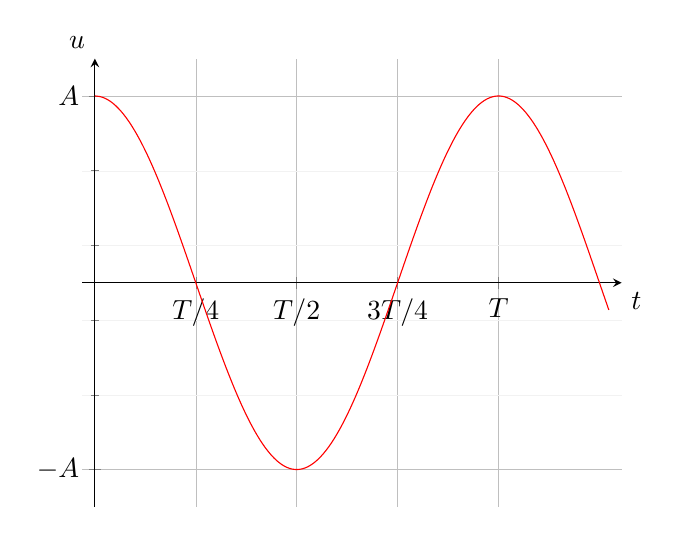
\begin{tikzpicture}
                \begin{axis}%
                    [grid=both,
                    minor tick num=4,
                    grid style={line width=.1pt, draw=gray!10},
                    major grid style={line width=.2pt,draw=gray!50},
                    axis lines=middle,
                    enlargelimits={abs=0.2},
                    xlabel={$t$},
                    ylabel={$u$},
                    xlabel style={below right},
                    ylabel style={above left},
                    xtick={pi/2,pi,3*pi/2, 2*pi},
                    xticklabels={$T/4$,$T/2$,$3T/4$,$T$},
                    ytick={-1,1},
                    yticklabels={$-A$,$A$}
                    ]
                    \addplot[domain=0:8,samples=100,smooth,red] {cos(deg(x))};
                \end{axis}
            \end{tikzpicture}
        \end{column}

        \begin{column}{0.4\textwidth}
            \begin{itemize}
                \item \(A\) é a amplitude
                \item \(T\) é o período e \(T=2\pi/\omega\)
                \item \(\omega\) é a frequência angular
                \item \(\omega t + \delta\) é a fase
                \item \(\delta\) é a constante de fase
                \item \(f\) é a frequência e \(\omega = 2\pi f\)
                    \[
                        \color{blue}
                        T=\frac{1}{f}
                    \]
            \end{itemize}
        \end{column}
    \end{columns}
\end{frame}

\begin{frame}{A constante de fase}
    \centering
    \begin{columns}[c]
        \begin{column}{0.45\textwidth}
            \[\delta = 0\]
            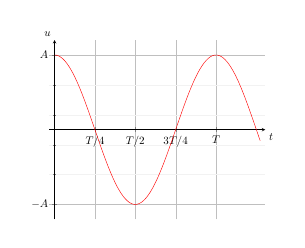
\begin{tikzpicture}[scale=0.4]
                \begin{axis}%
                    [grid=both,
                    minor tick num=4,
                    grid style={line width=.1pt, draw=gray!10},
                    major grid style={line width=.2pt,draw=gray!50},
                    axis lines=middle,
                    enlargelimits={abs=0.2},
                    xlabel={$t$},
                    ylabel={$u$},
                    xlabel style={below right},
                    ylabel style={above left},
                    xtick={pi/2,pi,3*pi/2, 2*pi},
                    xticklabels={$T/4$,$T/2$,$3T/4$,$T$},
                    ytick={-1,1},
                    yticklabels={$-A$,$A$}
                    ]
                    \addplot[domain=0:8,samples=100,smooth,red] {cos(deg(x))};
                \end{axis}
            \end{tikzpicture}

            \[\delta = \pi\]
            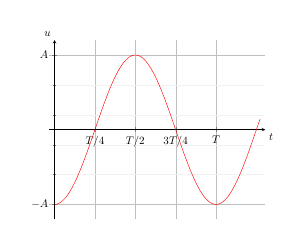
\begin{tikzpicture}[scale=0.4]
                \begin{axis}%
                    [grid=both,
                    minor tick num=4,
                    grid style={line width=.1pt, draw=gray!10},
                    major grid style={line width=.2pt,draw=gray!50},
                    axis lines=middle,
                    enlargelimits={abs=0.2},
                    xlabel={$t$},
                    ylabel={$u$},
                    xlabel style={below right},
                    ylabel style={above left},
                    xtick={pi/2,pi,3*pi/2, 2*pi},
                    xticklabels={$T/4$,$T/2$,$3T/4$,$T$},
                    ytick={-1,1},
                    yticklabels={$-A$,$A$}
                    ]
                    \addplot[domain=0:8,samples=100,smooth,red] {cos(deg(x+pi))};
                \end{axis}
            \end{tikzpicture}
        \end{column}

        \begin{column}{0.45\textwidth}
            \[\delta = \pi/2\]
            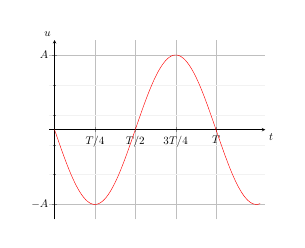
\begin{tikzpicture}[scale=0.4]
                \begin{axis}%
                    [grid=both,
                    minor tick num=4,
                    grid style={line width=.1pt, draw=gray!10},
                    major grid style={line width=.2pt,draw=gray!50},
                    axis lines=middle,
                    enlargelimits={abs=0.2},
                    xlabel={$t$},
                    ylabel={$u$},
                    xlabel style={below right},
                    ylabel style={above left},
                    xtick={pi/2,pi,3*pi/2, 2*pi},
                    xticklabels={$T/4$,$T/2$,$3T/4$,$T$},
                    ytick={-1,1},
                    yticklabels={$-A$,$A$}
                    ]
                    \addplot[domain=0:8,samples=100,smooth,red] {cos(deg(x+pi/2))};
                \end{axis}
            \end{tikzpicture}

            \[\delta = -\pi/2\]
            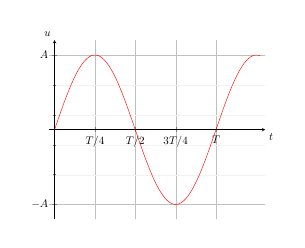
\begin{tikzpicture}[scale=0.4]
                \begin{axis}%
                    [grid=both,
                    minor tick num=4,
                    grid style={line width=.1pt, draw=gray!10},
                    major grid style={line width=.2pt,draw=gray!50},
                    axis lines=middle,
                    enlargelimits={abs=0.2},
                    xlabel={$t$},
                    ylabel={$u$},
                    xlabel style={below right},
                    ylabel style={above left},
                    xtick={pi/2,pi,3*pi/2, 2*pi},
                    xticklabels={$T/4$,$T/2$,$3T/4$,$T$},
                    ytick={-1,1},
                    yticklabels={$-A$,$A$}
                    ]
                    \addplot[domain=0:8,samples=100,smooth,red] {cos(deg(x-pi/2))};
                \end{axis}
            \end{tikzpicture}
        \end{column}
    \end{columns}
\end{frame}

\begin{frame}{Exemplos}
    \begin{itemize}
        \item Problemas 1 e 3
        \item Problemas 8, 12 e 16
    \end{itemize}
\end{frame}

\begin{frame}{Pêndulo simples}
    \begin{columns}[T]
        \begin{column}{0.4\textwidth}
            \begin{tikzpicture}[scale=1/2,
                ground/.style={fill,pattern=north east lines,draw=none,minimum width=0.3,minimum height=0.6}
                ]
                \draw [ground] (0,0) rectangle (10,1);
                \draw [thick] (0,0) -- (10,0);
                \draw [dotted,thick] (5,0) -- (5,-8);
                \draw [thick] (5,0) -- ++(-60:8) node [midway, above right] {L} node [circle, fill=blue!10, draw=black] {m} coordinate (A);
                \draw [red,->] (A) ++(0,-0.5) -- ++(0,-1) node [below] {mg} ;
                \draw (5,-2) arc (270:300:2) node [midway, below] {$\theta$};
            \end{tikzpicture}
        \end{column}
        \begin{column}{0.45\textwidth}
            \begin{itemize}
                \item Temos que \(\tau = -Lmg \sen{\theta}\)
                \item \textit{Lembrando de Física I}, temos que
                    \[
                        I\alpha = \tau \implies I\frac{d^2 \theta}{dt^2} = -Lmg\sen{\theta}
                    \]
                \item Quando \(\theta \to 0\) temos \(\sen{\theta} \to \theta\) e assim
                    \[
                        \frac{d^2\theta}{dt^2} = - \frac{Lmg}{I}\theta
                    \]
                \item Ou seja 
                    \begin{itemize}
                        \item para \(\theta\) grande não temos um MHS
                        \item para \(\theta\) pequeno temos um MHS
                    \end{itemize}
            \end{itemize}
        \end{column}

    \end{columns}
\end{frame}

\begin{frame}[c]{Pêndulo simples simplificado}
    Se pudermos considerar a massa do fio desprezível e a massa do corpo que oscila concentrada no centro de massa, temos que
    \(I=mL^2\) e assim temos a fórmula
    \[
        \omega = \sqrt{\frac{g}{L}}
    \]
\end{frame}

\begin{frame}{Casos especiais}
    \begin{itemize}
        \item Problemas 55 e 56
    \end{itemize}
    
\end{frame}
